\section{System Description} Havven is designed to incentivise stability in a decentralised cryptocurrency denominated in some external currency, such as the USD. The dual-token asset system is combined with a set of novel incentive mechanisms designed to stabilise the price of one of the two tokens. We refer to these as the havven token (\HAV{}) - to avoid confusion with the system itself - and the nomin, \NOM{} (short for denominator). \\

\noindent \HAV{} serves two functions:

\begin{enumerate}
\item{To provide the system with collateral (the system itself is tokenised), and,}
\item{To allow actors to contribute to the price stabilisation process through a set of incentives.}
\end{enumerate}

\noindent The second token, \NOM{}, is the stablecoin. The purpose of \NOM{} is to track the price of a chosen external denominating currency via the actions of \HAV{} token holders; holders of \HAV{} participate in modifying the level of supply in the \NOM{} market such that the market price of \NOM{} is maximally stable.

\subsection{Incentive Layering}

We classify the various incentives that can be applied in a stablecoin system. Note that any subset of these can be linearly combined in order to produce a sophisticated and powerful incentive structure. Havven's approach to achieving price stability is to be as passive as possible and only switch on higher levels of incentivisation when necessary. The order in which these categories appear is the order in which they are applied:

\paragraph{Overcollateralisation}

The basis for price stability within Havven is overcollateralisation of stablecoin value (i.e. the is a greater value in collateral backing the stablecoin than there is in the market capitalisation of all the \NOM{} in circulation. This ratio of \NOM{} to \HAV{} is known as the utilisation ratio.

\paragraph{Fees}

\noindent The second layer of economic incentives for \HAV{} holders is to provide them with earned fees in accordance with their performance in adjusting the supply of \NOM{}. These fees are generated from small charges on all \NOM{} transfers. These fees are directed to the \HAV{} holders as a reward for helping maintain the correct supply of \NOM{}.

\paragraph{Interest Rates}

\noindent Interest rates for \HAV{} can be applied in addition to the application of fees, in either fixed or floating \HAV{} supply regimes. Interest rates will be discussed in a future iteration of the whitepaper.

\paragraph{Collateral Recovery}

\noindent As a final layer of incentives, forced recovery of an actor's \HAV{} may be required in order to equilibriate individual positions of utilisation ratio. Collateral recovery will be discussed in a future iteration of the whitepaper.

\subsection{Overcollateralisation}

\noindent We first introduce the core system variables:

\begin{align*}
H &= \text{Quantity of \HAV{},} & N &= \text{Quantity of \NOM{},} \\
P_h &= \text{\HAV{} Price,}  & P_n &= \text{\NOM{} Price.}
\end{align*}

\noindent All \HAV{} tokens are created in the initial system state, so $H$ is constant. The quantity of \NOM{}, $N$, floats in response to the actions of havven holders, who, for the most part, are assumed to act in accordance with their incentives, thereby encouraging the \NOM{} price, $P_n$, to stabilise with changes in demand.

\subsubsection{Nomin Supply Control}

\noindent \NOM{} can only be issued when a \HAV{} holder decides to escrow some number of \HAV{} under their control. Once the \HAV{} have been escrowed (via smart contract) a quantity of \NOM{} are generated equal in value to the value of escrowed \HAV{} multiplied by the maximum utilisation ratio. This ensures the value of the \NOM{} that is produced is less than the value of the backing \HAV{} collateral. \\

\noindent Once the \HAV{} are escrowed, the system immediately places a \textbf{limit sell} order with a price of \$1 on an exchange (such as a dedicated decentralised exchange for havven and nomin trading). This means that the \NOM{} will be sold at the current market price, but with a minimum price of \$1 USD. If we assume implementation on Ethereum, then the \NOM{} are sold for an amount of ETH valued at \$1, with the proceeds of the sale remitted to the issuer. \\

\noindent It is important for the proper functioning of the system that the pool of \NOM{} is always overcollateralized by the value of \HAV{}. The \textbf{utilisation ratio} is what initialises this property.

\subsubsection{Utilisation Ratio}

\noindent The utilisation ratio is defined by the total value of \NOM{} against the total value of \HAV{}:

$$ U = \frac{P_n * N}{P_h * H} $$ \\

\noindent Intuitively, if $U = 1$, the value of \NOM{} and \HAV{} are equal. Hence, given our overcollateralisation property, our target $U <  1$. To do this, Havven only allows the issuance of \NOM{} up to a maximum utilisation ratio.

\subsubsection{Collateralisation Target}

\noindent Given the need to adjust the supply of \NOM{}, a target utilisation ratio is defined as the point at which maximum incentives are applied:

$$ 0 \leq U \leq U_{max} \leq 1.$$

\noindent Because individual havven holders have a unique utilisation ratio, $ U_i $, the system can measure the degree to which their $ U_i $ is above or below the target and adjust their incentives accordingly. In this way the system incentivises the creation and destruction of \NOM{}. $ U_{target} $ is defined formally below in terms of $ P_n $ (as \NOM{} price diverges from the desired \$1, increasing incentives are applied to either expand or contract the supply).

\subsubsection{Releasing Havvens from Escrow}

\noindent In order to access the original \HAV{} that have been escrowed, the owner must return the same quantity of issued \NOM{} to the system for destruction. This is known as 'burning' the \NOM{}.

\newpage
\subsection{Nomin Demand and Supply} 

\noindent Demand and supply economics shows that there exists some optimal supply of \NOM{} where the related level of demand yields an equilibrium price of \$1. We can express this quantity in terms of an optimum utilisation ratio, $U_{opt}$. The graph below visualises this situation. \\

\begin{figure}[h!]
    \centering
    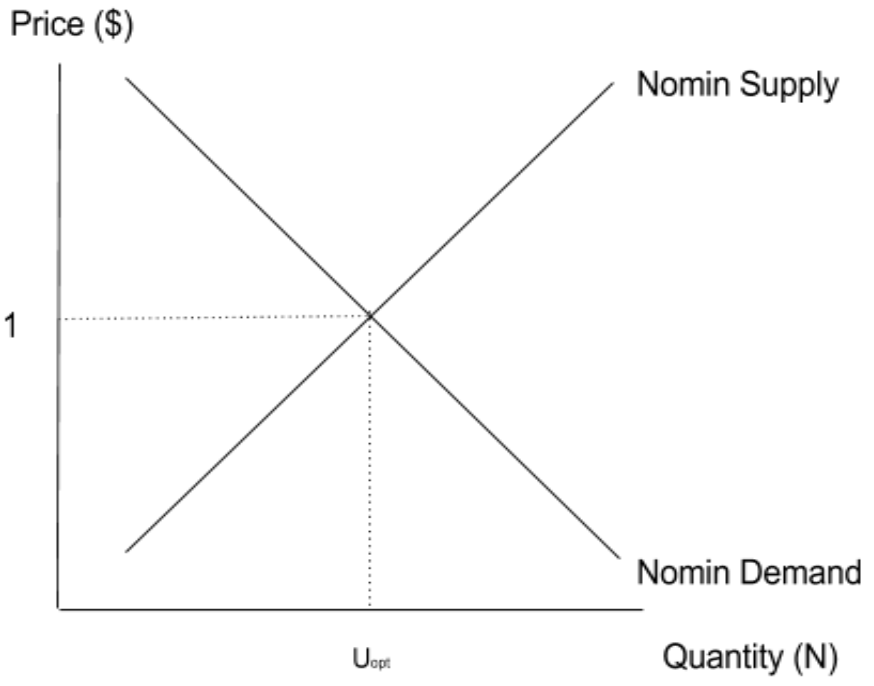
\includegraphics[width=.7\textwidth]{img/nomin-demand-vs-supply}
\end{figure}

\subsubsection*{Demand}

\noindent The system is unable to influence the demand for \NOM{}. We assume that some level of demand exists given the utility of nomins as a stable cryptocurrency.

\subsubsection*{Supply}

\noindent However where demand is unable to be directly influenced, the supply of \NOM{} is controlled by havven holders who use system levers to issue and burn \NOM{} in response to system incentives. Maximum incentive is achieved when $U_i = U_{opt}$, such that $P_n = 1$. $U_{opt}$ will be discussed further below. \\

\newpage
\subsection{Fees} Every time a Nomin transaction occurs, the Havven system charges a small transaction fee. Transaction fees allow the system to generate revenue, which it can distribute to \HAV{} holders as an incentive to maintain \NOM{} supply at $U_{opt}$.

\subsubsection{Transaction fees}

\noindent The fee charged on nomin transactions is constant and will be sufficiently small that it provides little to no friction for the user. \\

$$ a_c = k.$$

\begin{figure}[h!]
    \centering
    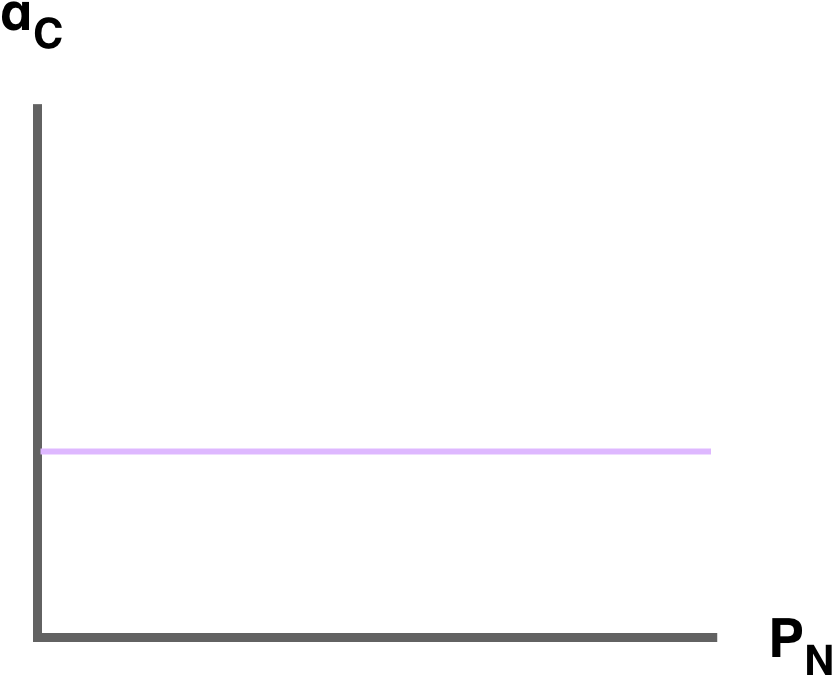
\includegraphics[width=.55\textwidth]{img/fees-charged}
\end{figure}

\newpage
\subsubsection{Fee distribution}

\noindent Fees are only paid to \HAV{} holders who have elected to escrow, as a reward for collateralising the system. The fees received increases linearly to a maximum at the optimal utilisation ratio $U_{opt}$. However, the fees quickly diminish as $U_I$ approaches $U_{max}$ before dropping to zero. \\

\[
\alpha_r = 
\begin{cases}
 \frac{\alpha_{base}}{U_{opt}} * U_I &\mbox{when } U_I \leq U_{opt}, \\ 
 \frac{\alpha_{base}}{U_{max} - U_{opt}} * (U_I  - U_{max}) &\mbox{when } U_{opt} \leq U_I \leq U_{max}, \\ 
 0 &\mbox{otherwise}.
 \end{cases}
\]

\begin{figure}[h!]
    \centering
    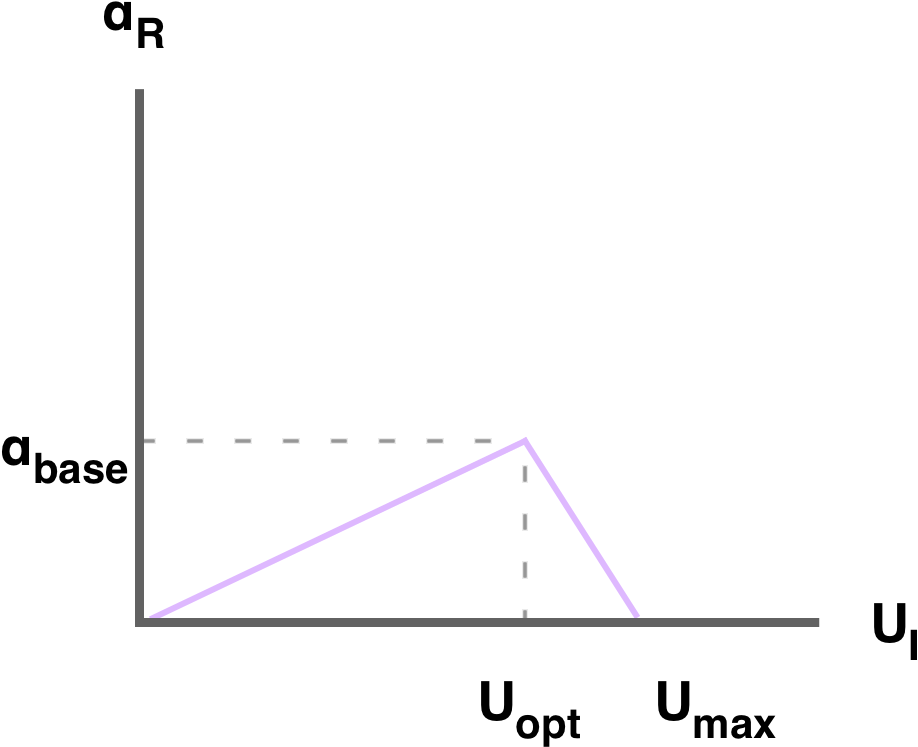
\includegraphics[width=.55\textwidth]{img/fees-received}
\end{figure}

\noindent This fee distribution curve encourages \HAV{} holders who have escrowed to maintain their $U_i$ at $U_{opt}$.  \\

\noindent We have introduced the concept of an optimal utilisation ratio and its importance in achieving $P_n = 1$. However, the system needs a function to determine what $U_{opt}$ is. \\

\noindent If $P_n > 1$ then the system must encourage more \NOM{} to be issued. If $P_n < 1$, the system must encourage \NOM{} to be burned. The definition of $U_{opt}$ must therefore provide this incentive.

\newpage
\subsubsection{Optimal Utilisation Ratio}

\noindent The optimal utilisation function given below provides us a dynamic target for havven holders based on the price of \NOM{}. The curve shows that the when $P_n$ is close to \$1, $ f'(P_n) $ is small. However, the further $P_n$ diverges from \$1, the larger the derivative becomes, providing an increasing incentive (via fees) for a havven holder to move toward $U_{opt}$ the further $P_n$ diverges from \$1.

$$ U_{opt} = f(P_n) * U,$$
$$ f(x) = max(\sigma * (x - 1)^{\phi} + 1, 0), $$
$$\text{where } 0 \leq \sigma, \text{ the price sensitivity parameter}, $$
$$\phi \geq 1, \text{ the flattening parameter}. $$ \\

\begin{figure}[h!]
    \centering
    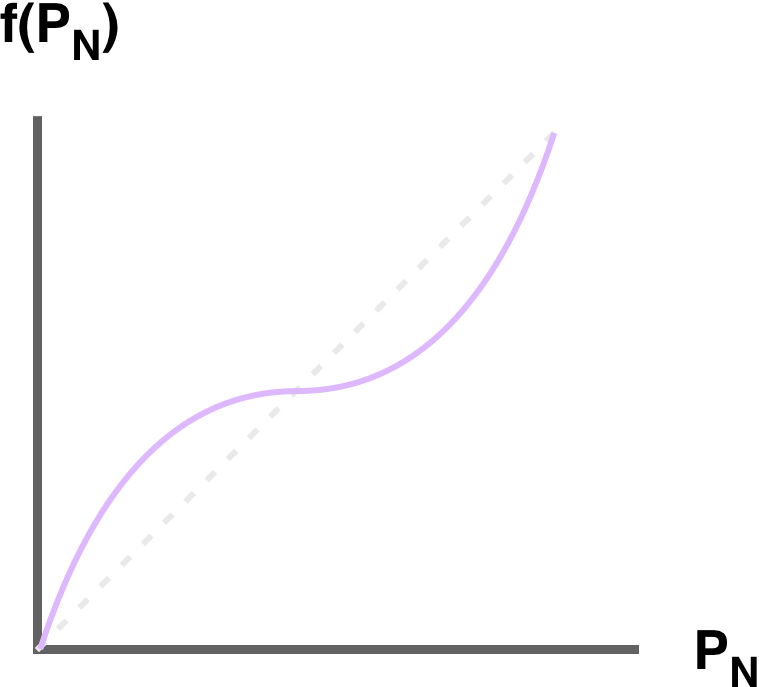
\includegraphics[width=.5\textwidth]{img/U_opt}
\end{figure}

\newpage

\subsection{Maximum Utilisation Ratio}

\noindent Havven seeks to maintain $U < U_{max} < 1$, in order to remain overcollateralised. It might seem intuitive that $U_{max}$ should be a static value. However, since $U_{opt}$ changes linearly with $P_n$ and inversely with $P_h$, there are several situations where $U_{max}$ may need to change. Below we define $U_{max}$. \\

\[
U_{max} = 
\begin{cases}
 U_{base} &\mbox{when } U_{opt} \leq U_{base}, \\ 
 \alpha * U_{opt} &\mbox{otherwise}. \\
 \end{cases}
\]

\begin{figure}[h!]
    \centering
    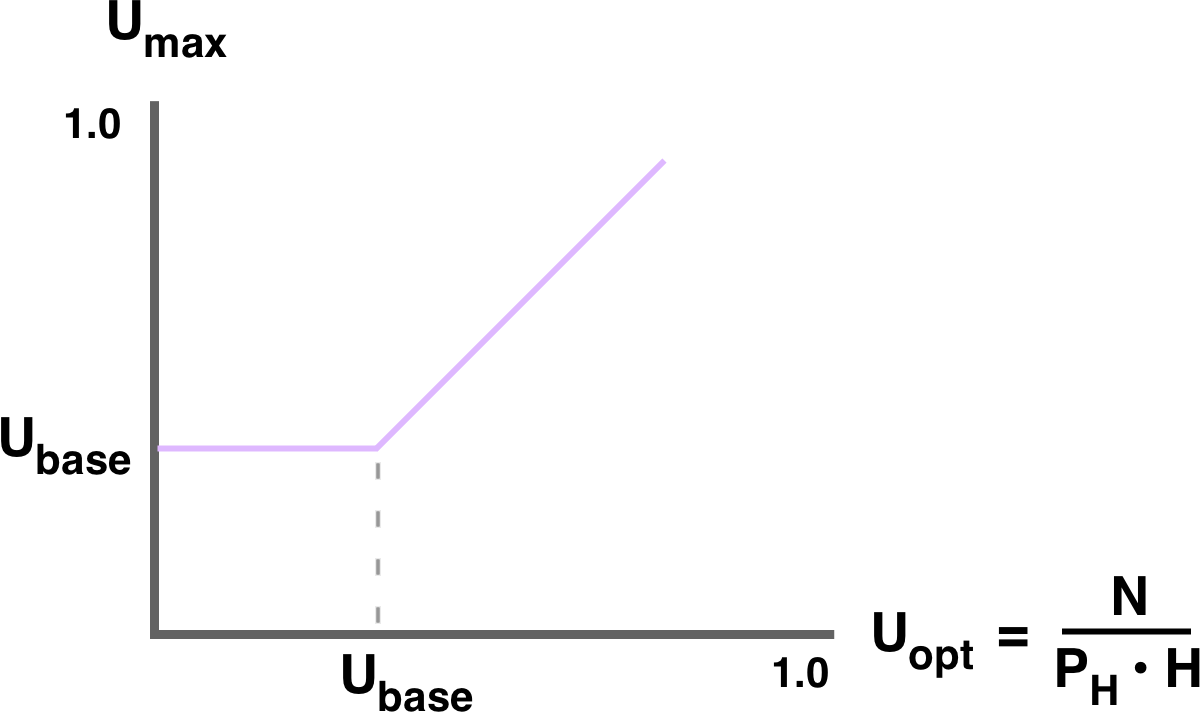
\includegraphics[width=.75\textwidth]{img/U_max}
\end{figure}

\newpage

\subsection{Intrinsic Havven Price} With the \HAV{} token being ERC20 compliant, it will have a market price on both decentralised and centralised exchanges. \\

\noindent While the Havven system will access the current market price via a price oracle, it is beneficial to define a $P_h$ that can be determined internally to avoiding the influence of speculation. Ignoring speculative demand, $P_h$ can be expressed as a function of the transaction fees that the system charges. Below we define an initial iteration of the intrinsic $P_h$.

\begin{align*} 
P_{h,t} &= \frac{1}{H}* \sum\limits_{t=1}^\infty \frac{d_{n,t} *v_{n,t} * \alpha_{R,t}}{(1+R)^t} \approx \frac{d_{n,t} *v_{n,t} * \alpha_{R,t}}{R * H}, \\
& P_{h,t} \text{ is the price of one \HAV{} at time } t, \\
& H \text{ is the number of havvens}, \\
& d_{n,t} \text{ is the demand for \NOM{} at t}, \\
& v_{n,t} \text{ is the velocity of \NOM{} at t}, \\
& \alpha_{R,t} \text{ is the fee from trade with \NOM{}}, \\
& R \text{ is the interest rate / rate of return of havvens}. \\
\end{align*}

\newpage
\subsection{Actor Definitions}
\paragraph{Havven Holder}
\emph{An investor who owns \HAV{} tokens.} \\

\noindent In order to purchase \HAV{} the expected return has to be greater than that of alternative investments (opportunity cost). The expected return of \HAV{} comes from:
\begin{enumerate}
\item{The fees received on escrowed \HAV{}.}
\item{An increase in $P_h$.}
\item{Seigniorage (i.e., an increment in $P_h$ implies that the investor can issue more \NOM{}, which may eventually have a larger value than his original investment.}
\end{enumerate}

\noindent At any moment in time, the investor must decide:
\begin{enumerate}
\item{Whether or not to issue new \NOM{} (assuming $U_i < U_{max}$), or to burn some of them. All \NOM{} are issued/burnt at the prevailing market exchange rate, denominated in ETH.}
\item{Whether to sell some quantity of \HAV{} in the market at price $P^M_{h,t}$. Only \HAV{} which haven't been escrowed can be sold. Otherwise they must burn \NOM{} to release them. }
\end{enumerate}

\paragraph{Nomin User}
\emph{A person who uses the Nomin token.} \\
 
\noindent In order to purchase \NOM{}, it must provide the user more utility than USD, since both have the same consumption value in the market. This utility may come from the properties of crypto. \\

\noindent At any time, they must decide: 
\begin{enumerate}
\item{Whether to buy or to sell \NOM{} at $P_n$.}
\end{enumerate}

\subsection{Example Use Case}

\noindent The issuance concept is best understood using an example:
\begin{enumerate}
\item{Bob owns 10 \HAV{} worth \$10 each, total value \$100.}
\item{The maximum utilisation ratio is 0.2.}
\item{Bob decides to escrow all of his \HAV{}, equivalent to 20 \NOM{}. These \HAV{} are now not able to be traded.}
\item{The system sells 20 \NOM{} on the market and transfers the proceeds, in ETH, to Bob's wallet.}
\item{Bob is free to use the ETH in his wallet in any way, including retaining it for the future purchase of \NOM{}.}
\item{In order to release the escrowed \HAV{}, the same number of \NOM{} (20) must be returned to the system, even if they have changed in value to say \$21 or \$19.}
\end{enumerate} 

\noindent Some questions may have already arisen in the reader's mind: \\

\noindent \emph{1. Does Bob have to lock all of his \HAV{} into escrow?} \\ 

\noindent There is no requirement for Bob to escrow all of his \HAV{}; he can escrow as many as he likes. The quantity of \NOM{} that is sold on the market is $ P_h * H_e * U_{max} $ where $H_e$ indicates the quantity of \HAV{} that was escrowed. \\

\noindent \emph{2.What if Bob would like to release his \HAV{}? Where would he acquire \NOM{}?} \\ 

\noindent He simply needs to purchase them in the open market. Assuming an implementation on Ethereum, \HAV{} and \NOM{} would both be ERC20-compatible tokens able to be traded on a variety of centralised and decentralised exchanges. Once Bob buys $20$ \NOM{}, he can present them to the system to be burned, thus releasing the escrowed \HAV{} back to him. \\ 

\noindent \emph{3. What happens if the price of \HAV{} changes?} \\

\noindent All issuance of \NOM{} is done at the current $P_h$. However, when $P_h$ changes, the quantity of escrowed \HAV{} changes with it (not the \emph{value}). An increase in $P_h$ means that fewer of Bob's \HAV{} are escrowed. By contrast, a decrease in the $P_h$ means that more of his \HAV{} are escrowed. This process occurs automatically in order to ensure that the system remains overcollateralised. \\ 

\noindent \emph{4. What happens if the price of \NOM{} changes?} \\ 

\noindent In order to release escrowed \HAV{}, Bob must return the same quantity of \NOM{} that he issued. This means that if $P_n$ has increased in the market, he will need to spend more ether than he received when he issued in order to release his \HAV{}. Conversely, if $P_n$ has decreased, Bob will need to spend less in order to release his \HAV{}.

\subsubsection{Havven Wallet}

\todo[inline]{add diagram of wallet balances.}

\newpage
